\documentclass[17pt]{beamer}
\usetheme{Warsaw}
\usefonttheme[onlymath]{serif}
\mode<all>
%\mode<article>{Extra detail mentioned only in the article version.}
%\mode<handout>{\setbeamercolor{background canvas}{bg=black}}
\usepackage[utf8]{inputenc}
\usepackage[TS1, T1]{fontenc}
\usepackage[french]{babel}
\usepackage{graphicx}
\geometry{papersize={165mm, 130mm}}%lmargin=0.8cm
\usepackage{amsmath, amssymb}
\usepackage{array}
\usepackage{fourier}
%%%%%%%%%%%%%%%%%%%%%%
%\usepackage{pgf}
\usepackage{pgfpages}
\pgfpagesuselayout{4 on 1}[a4paper, landscape, border shrink=.5cm]
%%%%%%%%%%%%%%%%%%%%%%%%%
%\setcounter{tocdepth}{1}
%%%%%%%%%%%%%%%%%%%%%%%%%%%%%
\newcommand{\abs}[1]{\lvert#1\rvert}
\newcolumntype{C}{>{$}c<{$}}
\newcounter{numsrc}
%%%%%%%%%%%%%%%%%%%%%%%%%%%%%%%%
\usepackage{listings}
\usepackage{fancyvrb, xcolor,fancyvrb-ex}
\newcommand\code{\fontsize{12}{6}\selectfont\color{blue!50!black}}
\fvset{formatcom=\code,  labelposition=bottomline, frame=lines}
\newcommand{\bleu}[1]{\textcolor{blue!75!black}{#1}}
%%%%%%\%%%%%%%%%%%%%%%%%%%%%%
\title{Introduction à \LaTeX}
\subtitle{L'essentiel pour écrire son document}
\author[clemsadand@gmail.com]{Clément ADANDE\\ clemsadand@gmail.com}
\institute[IMSP-UAC]{Université d'Abomey-Calavi\\%
%	\includegraphics[scale=0.4]{uac_logo}
%	~~~\raisebox{0.5cm}{
		Institut de Mathématiques et des Sciences Physiques
%	}
%	~~~\includegraphics[scale=.4]{logo_imsp}
}
%%%%%%%%
\setbeamertemplate{navigation symbols}{}
\setbeamercovered{transparent}%pour écrire le texte qui suit \pause en transparent
\setbeamerfont{title}{size=\Large,series=\bfseries}
\setbeamertemplate{itemize items}[circle]
\setbeamertemplate{enumerate items}[circle]
\setbeamertemplate{footline}[page number]
%\setbeamertemplate{normal text}{size=\Large}
%%%%%%%%%%%%%
\AtBeginSection[] % Do nothing for \section*
{
	\begin{frame}[plain]{Plan}
	\tableofcontents[currentsection,hideothersubsections]
	\end{frame}
}
%%%%%%%%%%%
\begin{document}

\begin{frame}[plain]
\maketitle
\end{frame}

\section*{Introduction}
\subsection{\LaTeX{}, c'est quoi ?}

\begin{frame}{\LaTeX{}, c'est quoi ? }
%Selon \href{url:https://fr.m.wikipedia.org/wiki/LaTeX}{Wikipédia}, <<\LaTeX{} est un langage et un système de composition de documents. Il s'agit d'une collection de macro-commandes destinées à faciliter l'utilisation du \textit{processeur de texte} \TeX{} de Donald Knuth.>>
\begin{block}{Généralité}
\LaTeX{} est un programme de compositions de textes. \LaTeX{} est beaucoup utilisé dans les domaines techniques et scientifiques pour réaliser plusieurs types de documents.
\end{block}
\end{frame}

\subsection{Pourquoi l'utilisé ?}

\begin{frame}{Pourquoi l'utilisé ?}
\begin{block}{Utilité}
\begin{itemize}
\item \LaTeX{} permet d'écrire du texte sans se soucier de la mise en page, d'écrire des formules mathématiques complexes sans grandes \textit{difficultés},\dots
\item \LaTeX{} dispose d'une documentation très vaste et est gratuit.
\end{itemize}
\end{block}
\end{frame}
%%%%%%%%%%
\begin{frame}[plain]{Sommaire}
\tableofcontents[hideallsubsections]
\end{frame}

\section{Fonctionnement et installation}
\subsection{Fonctionnement}

\begin{frame}{Fonctionnement}
%A la différence de Word et plein d'autre logiciel de traitement de textes, ce n'est pas ce que vous écrivez en \LaTeX}{} que vous obtenez dans votre document. 
\begin{block}{Le code source et sa compilation}
On compose son document \LaTeX{} en : 
\begin{enumerate}
\item écrivant un \bleu{code source} d'extension \bleu{.tex} ;
\item \bleu{compilant} son code source. 
\end{enumerate}
%Le résultat est fourni dans un format de description de pages propre à \TeX, DVI puis converti généralement en PDF.

Après la compilation un \LaTeX, un fichier \bleu{.pdf} est produit.
\end{block}
\end{frame}

\subsection{Installation}

\begin{frame}{Installation}
\framesubtitle{1}
\begin{block}{L'éditeur de textes et la distribution \TeX}
Pour utiliser \LaTeX, il suffit d'avoir :

\begin{enumerate}
\item \bleu{un éditeur de textes} : logiciel permettant d'écrire son code source \LaTeX et de visualiser son document ; 
\item \bleu{une distribution \TeX} :  ensemble de programmes permettant la compilation de son code source.
\end{enumerate}
\end{block}
\end{frame}

\begin{frame}{Installation}
\framesubtitle{2}
\begin{block}{Windows ou Linux}
\begin{itemize}
\item Sous Windows, on a le choix entre les distributions \TeX Live et MiK\TeX{} et sous Linux, la distribution \TeX Live est conseillé.
\item Par défaut, MiK\TeX{} installe lui-même son propre éditeur de textes, Texworks. On peut opter pour d'autres éditeurs comme Texstudio, Texmarker\dots
\end{itemize}
Pour installer ces programmes, rendez-vous le site de chaque projet.
\end{block}
\end{frame}

\section{Les bases}

\subsection{Premier source}

\begin{frame}[fragile]{Premier source}
\begin{block}{Notre premier document \LaTeX}
Ouvrez votre éditeur, copiez et compilez le code source ci-dessous.
\end{block}

\begin{Verbatim}%[label=source.tex]
\documentclass{article}
\begin{document}

Hello le public ! Je suis moi et vous êtes vous.

\end{document}
\end{Verbatim}
\end{frame}

\begin{frame}{Visualisation du document}
\includegraphics{firstdoc.pdf}
\end{frame}

\subsection{Différentes parties du source}

\begin{frame}[fragile]{Différentes parties du source}
\begin{block}{Le préambule et le corps}
\begin{itemize}
\item Un fichier source \LaTeX{} contient au minimum les trois commandes : \Verb+\documentclass{classeDeDocument}+, \Verb+\begin{document}+ et \Verb+\end{document}+. 
\item La partie qui précède \Verb+\begin{document}+ est appelée \bleu{préambule} ; 
\item La partie qui suit jusqu'au \Verb+\end{document}+ constitue le \bleu{corps} du document.% ; tout ce qui vient après \Verb+\end{document}+ est ignoré à la compilation.
\end{itemize}
\end{block}
\end{frame}

\begin{frame}{Hypothèses pour les autres exemples}
\begin{alertblock}{A votre attention}
Pour les autres fichiers sources proposés en exemple, on utilisera le même préambule que \Verb+source1.tex+ et pour gagner en espace, on écrira seulement le corps du document et on notifiera d'éventuelles instructions à ajouter au préambule en les précédent du caractère \Verb+*+.
\end{alertblock}
\end{frame}

\subsection{Caractères spéciaux}

\begin{frame}[fragile]{Caractères spéciaux}
%En observant le résultat du premier source, vous vous rendrez compte qu'il y a un grand nombre de choses qui sont dans le source et qui ne sont pas dans le pdf : ce sont des \textit{instructions}. 

%Certaines informations contenues dans le code source \LaTeX{} ne figure pas dans le document final : ce sont des \bleu{instructions}.
\begin{block}{Les dix caractères}
\begin{itemize}
\item On distingue deux catégories d'instructions en \LaTeX{} : les \bleu{commandes} et les \bleu{environnements}. 
\item Les caractères suivants servent à donner des instructions à \LaTeX{}.
\begin{center}
\Verb+\ { } _ ^ % & $ # ~+
\end{center}
%\item Le caractère \Verb+%+ permet de faire des commentaires.
\end{itemize}
\end{block}
\end{frame}

\subsection{Commandes et arguments}

\begin{frame}[fragile]{Commandes et arguments}
\framesubtitle{1}

\begin{block}{La syntaxe d'une commande}
\begin{itemize}
\item Une commande \LaTeX{} se présente comme suit :
\Verb+\commande[option1, option2,...,optionN]{argument1, argement2,...,argumentM}+
\item \textbf{Exemples : } \Verb+\documentclass{article}+, \Verb+\begin{document}+ et \Verb+\end{document}+ 
\end{itemize}
\end{block}
\end{frame}

\begin{frame}[fragile]{Commandes et arguments}
\framesubtitle{2}
 
\begin{block}{Exemple}
Copiez et compilez ce code source.
\end{block}
\begin{Verbatim}[label=source1.tex]
\documentclass[a4paper,12pt]{report}
\usepackage[utf8]{inputenc}
\usepackage[T1]{fontenc}
\usepackage[french]{babel}
\usepackage{amsmath, amssymb}
\newcommand{\abs}[1]{\lvert#1\rvert}%la valeur absolue
\begin{document}
Eh ! Ça y est ! Voici mon premier document \LaTeX. 

Soit $f$ une fonction numérique d'une variable réelle définie par : 

$f(x)=\sqrt{\abs{x^2-4}}+2x$.
\end{document}
\end{Verbatim}
\end{frame}

\begin{frame}[fragile]{Commandes et arguments}
\framesubtitle{3}
\begin{block}{Commandes utilisées précédemment}
%Voici ici quelques commandes utilisées dans l'exemple précédent.
\begin{center}
\begin{tabular}{|c|c|}\hline
\textbf{Commande} & \textbf{Rôle}\\\hline
\Verb+\documentclass+ & détermine l'apparence du document\\
\Verb+\usepackage+& permet de charger un paquet \\
\Verb+\newcommand+ & permet de définir de nouvelles commandes\\
\Verb+\sqrt+ & permet d'écrire sous radical\\
\Verb+\lvert+ et \Verb+\rvert+ & tracent des filets verticaux\\
\Verb+%+ & permet d'écrire un commentaire\\\hline
\end{tabular}
\end{center}
\end{block}
\end{frame}

\begin{frame}[fragile]{Paquet ou module}
\begin{block}{Les paquets}
\begin{itemize}
\item Un argument de la commande \Verb+\usepackage+ est appelé \bleu{module} ou \bleu{paquet}.
\item Il étend les possibilités de \LaTeX{} lorsqu'il est chargé.
\item \textbf{Exemples :} \Verb+inputenc+, \Verb+fontenc+, \Verb+babel+, \Verb+amsmath+, \Verb+amssymb+,\dots
\end{itemize}
\end{block}
\end{frame}

%\begin{frame}{Paquet ou module}
%\begin{block}

%\end{block}
%\begin{itemize}
%\item Les arguments de la commande \Verb+\usepackage+ sont appelés \bleu{modules} ou \bleu{paquets}. Lorsqu'ils sont chargés, ils étendent les possibilités de \LaTeX.
%\item Les paquets \Verb+inputenc+, \Verb+fontenc+ et \Verb+babel+ offrent respectivement la possibilité d'écrire des caractères accentués ; d'écrire des caractères accentués utilisés en Français et de calculer la coupure automatique des mots (avec l'option \Verb+T1+) ; et de traduire les titres en Français.
%\item Les paquets \Verb+amsmath+ et \Verb+amssymb+ étendent les possibilités d'écrire des expressions mathématiques en \LaTeX.
%%\item Pour éviter certains messages d'erreurs ou des résultats choquants à la compilation, veuillez à ce qu'au moins ces paquets soient tous chargés dans votre document.
%\end{itemize}
%\end{frame}


\subsection{Environnements}

\begin{frame}[fragile]{Environnements}
%Les commandes \Verb+\begin+ et \Verb+\end+ sont conjointement utilisées pour définir un environnement de la manière suivante.


\begin{block}{Synthaxe d'un environnement}
\begin{itemize}
\item Un environnement \LaTeX{} se présente comme suit :
\begin{BVerbatim}
\begin{environnement}[option1,option2,...optionN]{argument}
(contenu)
\end{environnement}
\end{BVerbatim}
\item \textbf{Exemple :} \Verb+{document}+
\end{itemize}
\end{block}
\end{frame}

\subsection{Messages d'erreur}

\begin{frame}{Messages d'erreur}
\begin{block}{Généralité}
\begin{itemize}
\item Lorsque la compilation ne se déroule pas bien, \LaTeX{} produit des messages d'erreur.
\item Il est important de \bleu{lire} et savoir \bleu{interpréter} les messages d'erreur.
\item \LaTeX{} indique souvent la ligne où se trouve l'erreur.
\item \LaTeX{} indique l'erreur mais pas toujours de façon explicite.
\end{itemize}
\end{block}
\end{frame}

\begin{frame}
\begin{block}{La correction des erreurs}
\begin{itemize}
\item Lisez le premier le message, corrigez l'erreur et compilez puis réitérez s'il y en a d'autres.
\item On peut commenter la ligne où se trouve l'erreur et revenir plus tard sur sa correction.
\item Copiez le message sur \href{http://www.google.com}{Google} et parcourez les blogs ou forums qui traitent du sujet. 
\item Consultez \cite{apl} à la page 44 ou rendez-vous sur l'adresse : \href{https://latex.developpez.com/cours/detecter-et-resoudre-les-erreurs/}{developpez.com}.
\end{itemize}
\end{block}
\end{frame}

\section{Le mode texte}

\subsection{Commandes}

\begin{frame}[fragile]{Quelques commandes}
%Le tableau suivant liste quelques commandes d'usage courant utilisées pour rédiger un document.
\begin{block}{Commandes couramment utilisées} 
\begin{center}
\begin{tabular}{|c|c|}\hline
\textbf{Commande} & \textbf{Rôle}\\\hline
\Verb+\textbf+ & met en \textrm{\textbf{gras}}\\
\Verb+\textit+ & met en \textrm{\textit{italique}}\\
\Verb+\textsl+& \textrm{\textsl{penche}}\\
\Verb+\underline+& \underline{souligne}\\
\Verb+\huge+& \textrm{\huge{agrandit}}\\
\Verb+\small+&\textrm{\small{diminue}}\\\hline
\end{tabular}
\end{center}
\end{block}
\end{frame}

\subsection{Espaces}

\begin{frame}[fragile]{Espaces}
\begin{block}{Les règles}
La gestion des espaces en \LaTeX{} est régis par quelques règles.
\begin{enumerate}
\item Les espaces au début d'une ligne sont ignorés.
\item Plusieurs espaces successifs sont équivalents à un seul espace.
\item Un retour à la ligne est équivalent à un espace.
\item Plusieurs lignes vides successives sont équivalentes à une seule ligne vide.
\end{enumerate}
\end{block}
\end{frame}

\begin{frame}[fragile]{Espaces}
\begin{block}{Le création d'espace}
\begin{itemize}
\item Les commandes \Verb+\hspace{(long)}+ et \Verb+\vspace{(long)}+ permettent créer des espaces horizontaux et verticaux de longueur \bleu{long}.
\item Le caractère \Verb+~+ crée un espace.
\end{itemize}
\end{block}
\end{frame}

\subsection{Les listes}

\begin{frame}[fragile]{Les listes}
\begin{block}{Les trois listes}
\begin{center}
\begin{tabular}{|c|c|}\hline
\textbf{Type de listes} & \textbf{Environnement}\\\hline
Les listes numérotées & \Verb+{enumerate}+ \\
Les listes à tirets & \Verb+{itemize}+ \\
Les listes de description & \Verb+{description}+ \\ \hline
\end{tabular}
\end{center}
La commande \Verb+\item+ permet de définir un élément de la liste.
\end{block}
\end{frame}

\begin{frame}[fragile]{Les listes}
\begin{block}{Exemple}
Copiez et compilez le source suivant.
\end{block}
\begin{Verbatim}[label=source2.tex]
\begin{enumerate}
\item liste numéroté
\item liste numéroté
\item liste numéroté
\end{enumerate}

\begin{itemize}
\item Jeux consoles
\item Jeux avec réalité augmenté
\item Billard
\end{itemize}

\begin{description}
\item[UAC] Université d'Abomey-Calavi
\item[Description] décrire
\item[Modalité] valeur possible
\end{description}
\end{Verbatim}
%\end{block}
\end{frame}

\subsection{L'alignement du texte}

\begin{frame}[fragile]{Alignement du texte}
\begin{block}{Les trois environnements}
\begin{center}
\begin{tabular}{|c|c|}\hline
\textbf{Environnement} & \textbf{Rôle}\\\hline
 \Verb+{center}+ & centre son contenu\\
 \Verb+{flushright}+ & aligne son contenu à gauche\\
 \Verb+{flushleft}+ & aligne son contenu à droite\\\hline
\end{tabular}
\end{center}
\end{block}
\end{frame}

\begin{frame}[fragile]{L'alignement du texte}
\begin{block}{Exemple}
Copiez et compilez ce code.
\end{block}

\begin{Verbatim}[label=source3.tex]
\begin{center}
Le texte est un test de mots remplies de structures grammaticales. Le présent
 se présente à tous. 
 
Sans plus tarder, ne tardons pas à terminer le travail.
\end{center}

\begin{flushright}
Le texte est un test de mots remplies de structures grammaticales. Le présent
 se présente à tous.
 
Sans plus tarder, ne tardons pas à terminer le travail.
\end{flushright}

\begin{flushleft}
Le texte est un test de mots remplies de structures grammaticales. Le présent
 se présente à tous.
 
Sans plus tarder, ne tardons pas à terminer le travail.
\end{flushleft}
\end{Verbatim}
\end{frame}

\subsection{Commandes de sectionnement}

\begin{frame}[fragile]{Classes de document}
\begin{block}{La classe de document}
\begin{itemize}
\item La classe de document détermine certains aspects de l'apparence du document. 
\item \textbf{Exemples :} \Verb+article+, \Verb+report+, \Verb+book+, \Verb+beamer+,\dots
%\item On utilise couramment les classes de document \Verb+article+, \Verb+report+ et \Verb+book+ respectivement pour les documents pas trop long, pour les documents de quelques dizaines de pages et pour réaliser des livres \cite{apl}. Un autre exemple de classes de document est \Verb+beamer+ utilisé pour réaliser des présentations (elle utilisé pour ce document).
%\item Chaque classe de document accepte une ou plusieurs options. Voici quelques options : \Verb+a4paper+, \Verb+openany+, \Verb+twocolumn+, \Verb+landscape+, \Verb+12pt+,  \Verb+11pt+ et  \Verb+10pt+. Pour rendre compte de leur effet sur le document, vous pouvez les tester.
\end{itemize}
\end{block}
\end{frame}

\begin{frame}[fragile]{Commandes de sectionnement}{1}
\begin{block}{Les commandes de sectionnement}
Les commandes de sectionnement sont utilisées pour gérer la structure du document : partie, chapitre, section, sous-section, sous-sous-section, paragraphe, sous-paragraphe, appendice,\dots
\end{block}
\end{frame}

\begin{frame}[fragile]{Commandes de sectionnement}{2}
\begin{block}{La classe article}
En classe \Verb+article+, la structure du document est la suivante.
\begin{BVerbatim}
\part{(titre de partie)}
\section{(titre de section)}
\subsection{(titre de sous-section)}
\subsubsection{(titre de sous-sous-section)}
\paragraph{(titre de paragraphe)}
\subparagraph{(titre de sous-paragraphe)}
\appendix
\section{(titre d’appendice)}
\section{(titre d’appendice)}
\end{BVerbatim}
\end{block}
\end{frame}

\begin{frame}[fragile]{Commandes de sectionnement}{3}
\begin{block}{Les classes book et report}
Les classes \Verb+report+ et \Verb+book+ utilisent en plus de tous les commandes de sectionnement de la classe \Verb+article+, la commande \Verb+\chapter{(titre de chapitre)}+ entre \Verb+\part+ et \Verb+\section+.
\end{block}
\end{frame}

\begin{frame}[fragile]{Commandes de sectionnement}{Exemple}
\begin{Verbatim}[label=source12.tex]
\documentclass[a4paper,12pt]{report}
\usepackage[utf8]{inputenc}
\usepackage[T1]{fontenc}
\usepackage[french]{babel}
\usepackage{amsmath, amssymb}
\newcommand{\abs}[1]{\lvert#1\rvert}%la valeur absolue
\title{Algèbre linéaire}%définit titre du document
\author{Clément A.\\ Etudiant en MFA1}%définit le nom de l'auteur
\date{\today}%définit une date, la commande \today donne la date aujourd'hui
\begin{document}
\maketitle%Permet d'afficher le titre, le nom et la date au début du document

\chapter{Espaces vectoriels}
\section{Généralités}

\subsection{Définition}

Soit E un ensemble muni non vide muni d'une loi de composition interne +
et d'une loi de composition externe $\cdot$. On dit que E est un espace
vectoriel lorsque\dots

\subsection{Sous-espaces vectoriels}
Un sous-ensemble d'un espace vectoriel est appelé sous-espace vectoriel \dots
\end{document}
\end{Verbatim}
\end{frame}

%\subsection{Paquets u}
%
%\begin{frame}{Le paquet geometry}
%Le module \Verb+geomtry+ permet de modifier la taille des marges, de la page
%\end{frame}


\section{Images et tableaux}

\subsection{Images}

\begin{frame}[fragile]{Insertion d'image}{1}

\begin{block}{Le paquet graphicx}
\begin{itemize}
\item Le paquet \Verb+graphicx+ permet d'inclure des photos son document.
\item La commande \Verb+\includegraphics[scale=prop]{image}+ place dans le paragraphe courant l'image \bleu{image} à l'échelle \bleu{prop}.
\item L'échelle est un nombre compris entre 0 et 1.
\item \alert{L'image et le fichier \Verb+.tex+ doivent être dans le même dossier ; sinon on indique l'endroit où elle se trouve.}
\end{itemize}
\end{block}
\end{frame}

\begin{frame}[fragile]{Insertion d'image}{2}
\begin{block}{Exemple}
Copiez et compilez ce code source.
\end{block}
\begin{Verbatim}[boxwidth=auto, label=source4.tex]
*\usepackage{graphicx}
L'oiseau de mon\dots
\begin{center}
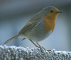
\includegraphics[scale=0.5]{oiseau}
\end{center}
\end{Verbatim}

\end{frame}

\subsection{Tableaux}

\begin{frame}[fragile]{Tableaux simples}{1}
\begin{block}{L'environnement tabular}
\begin{itemize}
\item L'environnement \Verb+{tabular}+ permet de construire un tableau.
\item Son argument est une suite finie formée avec les lettres \bleu{l}, \bleu{c} et \bleu{r} qui aligne à gauche, centre et aligne à droite le contenu de chaque colonne.
\item Le nombre de colonnes est égal au nombre d'éléments de cette suite.
\item Deux cellules sont séparées avec le caractère \Verb+&+.
\end{itemize}
\end{block}
\end{frame}


\begin{frame}[fragile]{Tableaux simples}{2}
%\begin{block}{Exemple}
\begin{Example}[boxwidth=auto, label=source5.tex]
\begin{tabular}{lcclr}
Animaux & Oiseaux & Chats & Moutons & Serpents\\
Effectif & 13 & 4 & 6& 11\\
\end{tabular}
\end{Example}
\end{frame}

\begin{frame}[fragile]{Tableaux simples}
\begin{block}{Les filets}
\begin{itemize}
\item Deux lignes sont séparées par la commande \Verb+\\+.
\item La commande \Verb+\hline+ trace un filet horizontal.
\item Le caractère \Verb+|+ trace un filet vertical.
\end{itemize}
\end{block}
\end{frame}

\begin{frame}[fragile]{Tableaux simples}{4}
\begin{Example}[label=source6.tex]
\begin{tabular}{|l|c|c|r|c|l|}
\hline Animaux & Oiseau & Chat & Moutons & Serpents\\
\hline Effectifs & 13 & 4 & 6 & 11\\
\hline Vendeurs & Jo & Fred & Egbéwè & Mike & Ledi \\
\hline
\end{tabular}
\end{Example}
%\end{block}
\end{frame}

\section{Les modes mathématiques}
\subsection{Les modes mathématiques}

\begin{frame}[fragile]{Deux modes : en ligne et hors-texte}{1}
\begin{block}{Les deux modes mathématiques}
\begin{itemize}
\item Le mode mathématique permet d'écrire des expressions mathématiques.
\item On distingue deux modes mathématiques : le mode \bleu{en ligne} et le mode \bleu{hors-texte}.
\item Ici, les espaces sont ignorés et les lettres sont écrites en italiques.
\item Aussi, la commande \Verb+\text{(textes)}+ permet d'écrire du texte.
\item Enfin, le caractère \Verb+~+ permet de créer un espace.
\end{itemize}
\end{block}
\end{frame}


\begin{frame}[fragile]{Les modes mathéquatiques}{2}

\begin{block}{En ligne ou hors-texte}
\begin{itemize}
\item \Verb+$...$+ délimite le mode en ligne et intègre son contenu au paragraphe en cours.
\item \Verb+\[...\]+ délimite le mode hors-texte et centre son contenu sur une nouvelle ligne.
\end{itemize}
\end{block}
\end{frame}


\begin{frame}[fragile]{Les modes mathématiques}{3}
\begin{block}{Exemple}
Copiez et compilez ce code source.
\end{block}
\begin{Verbatim}[label=source7.tex]
On appelle racine carrée de d'un nombre positif $x$, le nombre noté $\sqrt{x}$
et vérifiant : \[(\sqrt{x})^2=x.\]
On sait que : \[\abs{x}=x si x\geq 0.\]
\end{Verbatim}
\end{frame}

\subsection{Commandes mathématiques}

\begin{frame}[fragile]{Commandes mathématiques}
%\parbox{0.4\linewidth}{
%Le tableau ci-contre liste quelques commandes d'usage courant en mathématiques. 
%
%Le fichier \cite{tsm} contient une liste plus détaillée (mais non exaustive) de symboles mathématiques.

%En mode en ligne, les commandes \(\Verb+\sum+\) et \(\Verb+\lim+\) s'utilisent de la manière suivante : \(\Verb+\sum\limits_{k=0}^{n} k+\) et \(\Verb+\lim\limits_{x\to 0} f(x)+\). On les force ainsi à placer l'exposant et l'indice  respectivement au dessus et au-dessous de $\sum$et $\lim$.
\begin{block}{Commandes couramment utilisées en maths}
\begin{center}
\begin{tabular}{|C|c||C|c|}\hline
\text{\textbf{Résultat}} & \textbf{Code}&\text{\textbf{Résultat}} & \textbf{Code}\\\hline
2\times 6& \Verb+2\times 6+ & x\leq 6 & \Verb+x\leq -6+\\
x^{a} & \Verb+x^{a}+& x\geq 0 & \Verb+x\geq 0+\\
x_{i}& \Verb+x_{i}+ & x\neq y & \Verb+x\neq y+\\
\frac{a}{b} & \Verb+\frac{a}{b}+&\sum\limits_{k=0}^{n} k & \Verb+\sum_{k=0}^{n} k +\\
\sqrt[4]{67} & \Verb+\sqrt[4]{67}+&\displaystyle\int_{-1}^{1} f(x) dx & \Verb+\int_{-1}^{1} f(x) dx+\\
x\in \mathbb{R} & \Verb+x \in \mathbb{R}+ & \lim\limits_{x\to -\infty} f(x) & \Verb+\lim_{x\to -\infty} f(x)+\\
A\cup B& \Verb/A\cup B/&\displaystyle{\bigcup_{n=0}^{+\infty} A_n} & \Verb-\bigcup_{n=0}^{+\infty} A_n-\\
A\cap B & \Verb/A\cap B/ & \displaystyle{\bigcap_{n=0}^{+\infty} A_n} & \Verb-\bigcap_{n=0}^{+\infty} A_n-\\\hline
\end{tabular}
\end{center}
\end{block}
\end{frame}

\subsection{Environnements mathématiques}
\subsubsection{Alignement}
\begin{frame}[fragile]{Alignement}{1}
\begin{block}{L'alignement des formules}
%Pour aligner des expressions mathématiques, on utilise l'environnement \Verb+{aligned}+.
\begin{itemize}
\item L'environnement \Verb+{aligned}+ permet d'aligner des formules sur plusieurs.
\item Il est similaire à l'environnement \Verb+{tabular}+
\item \Verb+&+ et \Verb+\\+ jouent les mêmes rôles que pour l'environnement \Verb+{tabular}+.
\end{itemize}
\end{block}
\end{frame}

\begin{frame}[fragile]{Alignement}{2}
\begin{block}{Exemple}
Copiez et compilez ce code source.
\end{block}
\begin{Verbatim}[label=source8.tex]
\begin{enumerate}
\item Développons et réduisons $(x-1)^3$.

$\begin{aligned}
(x-1)^3 &= (x-1)(x-1)^2\\
        &=(x-1)(x^2-2x+1)\\
        &=x^3-2x^2+x-x^2+2x-1\\
        &=x^3-3x^2+3x-1
\end{aligned}$

\item Résoudre l'équation $x^3-3x^2+3x-1=0$ dans $\mathbb{R}$.

\[\begin{aligned}
x^3-3x^2+3x-1=0 &\iff (x-1)^3=0\\
                &\iff x-1=0\\
                &\iff x=1
\end{aligned}\]

L'ensemble des solutions de l'équation est $\{1\}$.
\end{enumerate}
\end{Verbatim}
\end{frame}

\subsubsection{Systèmes}

\begin{frame}[fragile]{Systèmes}{1}
%Pour écrire un système, on utilise l'environnement \Verb+{case}+.
\begin{block}{Les systèmes}
\begin{itemize}
\item L'environnement \Verb+{case}+ permet d'écrire des systèmes.
\item Il est similaire à l'environnement \Verb+{aligned}+.
\end{itemize}
\end{block}
\end{frame}

\begin{frame}[fragile]{Systèmes}{2}
\begin{Example}[label=source9.tex]
On considère la fonction définie par :
\[\begin{cases}
f(x) &= 2^{x^2-1} \text{ si } x>0\\
f(x) &= 0 \text{ si } x=0
\end{cases}\]
Etudier la continuité de $f$ en $0$.
\end{Example}
\end{frame}

\subsubsection{Matrices}

\begin{frame}[fragile]{Matrices}{1}
%Pour définir une matrice, on utilise l'environnement \Verb+{pmatrix}+.
\begin{block}{Les matrices}
\begin{itemize}
\item L'environnement \Verb+{pmatrix}+ permet d'écrire des systèmes. 
\item Il est similaire à l'environnement \Verb+{tabular}+.
\item L'environnepent \Verb+{vmatrix}+ permet d'écrire un déterminant.
\item Il s'utilise de la même manière que \Verb+{pmatrix}+.
\end{itemize}
\end{block}
\end{frame}

\begin{frame}[fragile]{Matrices}{2}
\begin{Example}[label=source10.tex]
Déterminer le rang de la matrice M.

\[M=\begin{pmatrix}
1 & 25 & 0 & 3\\
2 & 0 & 10 & 9\\
1 & 8 & 4  &-3
\end{pmatrix}.\]
\end{Example}
\end{frame}

\subsubsection{Formules numérotées}

\begin{frame}[fragile]{Formules numérotées}{1}
\begin{block}{L'environnement equation}
\begin{itemize}
\item L'environnement \Verb+{equation}+ permet de numéroté des expressions.% écrite en mode hors-texte.
\item Il permet aussi de faire référence à ces expressions n'importe où dans le document.
\item \alert{Il entre le mode mathématique hors-texte.}
\item La commande \Verb+\label{nom-ref}+ permet de marquer un endroit dans le document.
\item Les commandes \Verb+\eqref{nom-ref}+ et \Verb+\pageref{nom-ref}+ permettent de se référer au numéro ou page de cet endroit \Verb+nom-ref+.
\end{itemize}
\end{block}
\end{frame}

\begin{frame}[fragile]{Formules numérotées}{2}
\begin{Example}
On appelle système différentiel linéaire sur un intervalle réel I,
tout équation de la forme :
\begin{equation}
\label{sys-l}
X'(t)=A(t)X(t)
\end{equation}
où $A:t\in I\mapsto A(t)\in M_n(\mathbb R)$ une application continue.

L'ensemble des solutions du système linéaire \eqref{sys-l} est
un espace vectoriel de dimension $n$.
\end{Example}
\end{frame}

\subsection{Délimiteurs}

\begin{frame}[fragile]{Délimiteurs}{1}
\begin{block}{Les délimiteurs}
\begin{itemize}
\item Les caractères \Verb+(+, \Verb+|+ et \Verb+[+ sont des délimiteurs.
\item La commande \Verb+\{+ donne le délimiteur \Verb+{+.
\item Les commandes \Verb+\left+, \Verb+\middle+ et \Verb+\right+ ajustent les délimiteurs à la taille de leur contenu.
\item Une occurence de la commande \Verb+\left+ exige aussi celle de la commande \Verb+\right+.
\end{itemize}
\end{block}
\end{frame}

\begin{frame}[fragile]{Délimiteurs}{2}
\begin{Example}[label=source11.tex]
Montrer que l'ensemble 
\[E = \left\{\frac{n+1}{n+2}\middle| n\in\mathbb{N} \right\} \]
est borné. 

Le point de couple de coordonnées $\left(\frac{1}{4},-\frac{3}{4}\right)$ 
appartient à la droite d'équation $3x-y=0$. Donc on a :

\[
A(a,b)=-3\left[ \left(a-\frac{3}{7}\right)^2-\left(\frac{3}{7}\right)^2+b\right]
\]
\end{Example}
\end{frame}

\subsection{Environnements numérotés}

\begin{frame}[fragile]{Environnements numérotés}{1}
\begin{block}{Le paquet amsthm}
\begin{itemize}
\item Le module \Verb+amsthm+ permet de créer ses propres environnements et ils sont numérotés par définition. 
\item Consultez \cite{apl} à la page 41 ou téléchargez sa documentation à l'adresse \href{http:www.ctan.org/pkg/amsthm}{www.ctan.org/pkg/amsthm}.
\end{itemize}
\end{block}
\end{frame}

\begin{frame}[fragile]{Environnements numérotés}{2}
\begin{Verbatim}[label=source13.tex, labelposition=topline]
\documentclass{article}
\usepackage[utf8]{inputenc}
\usepackage[T1]{fontenc}
\usepackage[french]{babel}
\usepackage{amsthm}
\newtheorem{definition}{Définition}[section]%creation de l'environnement definition
\newtheorem{propriete}{Propriété}%propriete sera numeroté seul
\newtheorem{exemple}{Exemple}[definition]%exemple sera numeroté dans definition
\begin{document}
\section{Environnements numérotés}

\begin{definition}[Inverse]
On appelle inverse d'un nombre réel non nul $a$ le nombre $\frac{1}{a}$.
\end{definition}

\begin{exemple}
$\frac{1}{\sqrt{2}}$ est l'inverse de $\sqrt{2}$.
\end{exemple}

\begin{propriete}[de Pythagore]
Dans un triangle rectangle, le carré de l'hypoténuse est la somme des carrés
des longueurs des deux autres côtés.
\end{propriete}

\begin{exemple}
ABC est un triangle rectangle en A tel que : $AB=30$ et $BC=50$. Déterminer AC.
\end{exemple}
\end{document}
\end{Verbatim}
\end{frame}

\section{Quelques paquets supplémentaires}

\subsection{Le paquet hyperref}

\begin{frame}[fragile]{Références croisées}{1}
\begin{block}{Une référence croisée}
\begin{itemize}
\item Une référence renvoie d'un endroit à un autre dans le document.
\item La commande \Verb+\label{etiquette}+ permet de marquer un endroit.
\item La commande \Verb+\ref{etiquette}+ permet d'y référer plus tard.
\item \alert{Une étiquette est une suite finie de lettres différents des noms prédéfinis par \LaTeX{}.}
\item L'appel de la commande \Verb+\ref{etiquette}+ produit un numéro en fonction de la commande ou l'environnement numéroté qui \textit{contient} la commande \Verb+\label{etiquette}+.
\end{itemize}
\end{block}
\end{frame}

\begin{frame}[fragile]{Références croisées}{2}
\begin{Verbatim}
\documentclass{article}
\usepackage[utf8]{inputenc}
\usepackage[T1]{fontenc}
\usepackage[french]{babel}
\usepackage{amsthm}
\newtheorem{definition}{Définition}[section]%creation de l'environnement definition
\newtheorem{propriete}{Propriété}%propriete sera numeroté seul
\newtheorem{exemple}{Exemple}[definition]%exemple sera numeroté dans definition
\begin{document}
\section{Environnements numérotés et références croisées}

\begin{definition}[Inverse]
On appelle inverse d'un nombre réel non nul $a$ le nombre $\frac{1}{a}$.
\end{definition}

\begin{exemple}\labe{invfrac}
$\frac{1}{\sqrt{2}}$ est l'inverse de $\sqrt{2}$.
\end{exemple}

\section{Exercices}

A partir de l'exemple~\ref{invfrac}, donner quinze nombres et leurs inverses.
\end{document}
\end{Verbatim}
\end{frame}

\begin{frame}{Hyperliens}
\begin{block}{Le paquet hyperref}
\begin{itemize}
\item Le paquet \Verb+hyperref+ permet de créer des liens vers une destinatuon.
\item La commande \Verb-\href{argument1}{argument2}- crée un lien vers une destination.
\end{itemize}
\end{block}
\end{frame}

\subsection{Le paquet geometry}

\begin{frame}[fragile]{Structure de la page}
\begin{block}{La géométrie d'une page}

\end{block}
\end{frame}

\subsection{Le paquet fancyhdr}

\begin{frame}[fragile]{En-tête et pieds de la page}
\begin{block}{L'en-tête et le pieds de la page}

\end{block}
\end{frame}

\section*{Conclusion}

\begin{frame}{Conclusion}
\begin{block}{La conclusion}
\LaTeX{} est un champ très vaste qu'on ne peut entièrement explorer dans quelques dizaines de slides. Néanmoins, il dispose d'une très grande documentation qui rend son apprentissage un peu \textit{facile}. Pensez à \href{http:google.com}{Google} chaque fois que vous aurez besoin d'être dépanné et soyez patient.
\end{block}
\end{frame}
%%%%%%%%%%%%%%%%%%%
%%%%%%%%%%%%%%%%%%%%%%
\begin{frame}[plain]{Références}
\begin{thebibliography}{0}
\bibitem{apl} \emph{Apprentissage et pratique de \LaTeX{}}, Manuel \bsc{Pégourié-Gonnard},  1\up{er} semestre 2008-2009
\bibitem{wik} \emph{Latex}, \href{url:https://fr.wikipedia.org/wiki/LaTeX}{https://fr.wikipedia.org/wiki/LaTeX}
\bibitem{ctan} \emph{CTAN}, \href{http:ctan.org}{ctan.org}, site sur lequel vous trouverez toutes sortes de matériels autour de \TeX.
\bibitem{tsm} \emph{Tables de symboles mathématiques}, \href{http://people.math.jussieu.fr/~mpg/lm204/files/doc-symboles-math.pdf}{http://people.math.jussieu.fr/~mpg/lm204/files/doc-symboles-math.pdf}
\bibitem{dev} \emph{Détecter et résoudre les problèmes - \LaTeX{}}, \href{https://latex.developpez.com/cours/detecter-et-resoudre-les-erreurs/}{https://latex.developpez.com/cours/detecter-et-resoudre-les-erreurs/}
\end{thebibliography}
\end{frame}

\end{document}
